\documentclass[letter,12pt]{article}

\usepackage[T1]{fontenc}
% Nicer default font (+ math font) than Computer Modern for most use cases
\usepackage{mathpazo}
\usepackage{graphicx}
\usepackage{xcolor} % Allow colors to be defined
\usepackage{enumerate} % Needed for markdown enumerations to work
\usepackage{geometry} % Used to adjust the document margins
\usepackage{amsmath} % Equations
\usepackage{amssymb} % Equations
% The hyperref package gives us a pdf with properly built
% internal navigation ('pdf bookmarks' for the table of contents,
% internal cross-reference links, web links for URLs, etc.)
\usepackage{hyperref}
\usepackage{natbib}
\usepackage[scr]{rsfso}
\usepackage{bm}
\usepackage{mathtools}
\usepackage{pdflscape}
\usepackage[doublespacing]{setspace}
\usepackage{authblk}

% Colors for the hyperref package
\definecolor{urlcolor}{rgb}{0,.145,.698}
\definecolor{linkcolor}{rgb}{.71,0.21,0.01}
\definecolor{citecolor}{rgb}{.12,.54,.11}

\title{
    A Bayesian Non-parametric Approach to Geographic Regression Discontinuity Designs:
    Do School Districts Affect NYC House Prices?
}

\author[a]{Maxime Rischard}
\author[a]{Zach Branson}
\author[b]{Luke Miratrix}
\author[c]{Luke Bornn}
\affil[a]{Department of Statistics, Harvard University}
\affil[b]{Graduate School of Education, Harvard University}
\affil[c]{Simon Fraser University}

\DeclarePairedDelimiter{\parenthesis}{\lparen}{\rparen}
\DeclarePairedDelimiter{\squarebracket}{\lbrack}{\rbrack}
\DeclarePairedDelimiter{\curlybracket}{\lbrace}{\rbrace}
\DeclarePairedDelimiter{\absolutevalue}{\lvert}{\rvert}
\newcommand{\del}[1]{\parenthesis*{#1}}
\newcommand{\sbr}[1]{\squarebracket*{#1}}
\newcommand{\cbr}[1]{\curlybracket*{#1}}
\newcommand{\abs}[1]{\absolutevalue*{#1}}
\DeclareMathOperator{\dif}{d}
\DeclareMathOperator*{\argmin}{arg\,min}
\DeclareMathOperator*{\argmax}{arg\,max}
\let\Pr\relax
\DeclareMathOperator{\Pr}{\mathbb{P}}
\DeclareMathOperator{\E}{\mathbb{E}}
\DeclareMathOperator{\V}{\mathbb{V}}
\DeclareMathOperator{\cov}{{Cov}}
\DeclareMathOperator{\var}{{var}}
\DeclareMathOperator{\Ind}{\mathbb{I}}
\DeclareMathOperator*{\sgn}{{sgn}}

\DeclareMathOperator{\normal}{\mathcal{N}}
\DeclareMathOperator{\unif}{Uniform}
\DeclareMathOperator{\invchi}{\mathrm{Inv-\chi}^2}
\DeclareMathOperator{\ones}{\mathbf{1}}
\DeclareMathOperator{\GP}{\mathcal{GP}}
\newcommand{\building}{\mathtt{BuildClass}}
\newcommand{\district}{\mathtt{Distr}}

\newcommand*{\trans}{^{\mkern-1.5mu\intercal}}
% \newcommand{\trans}{^{\top}}

\newcommand{\area}{\mathcal{A}}
\newcommand{\treat}{\mathrm{T}}
\newcommand{\ctrol}{\mathrm{C}}
\newcommand{\treatind}{Z}
\newcommand{\treatarea}{\area{}^{\treat}}
\newcommand{\ctrolarea}{\area{}^{\ctrol}}

\newcommand{\sigmaf}{\sigma_{\mathrm{GP}}}
\newcommand{\sigman}{\sigma_{\epsilon}}
\newcommand{\sigmabeta}{\sigma_{\beta}}
\newcommand{\sigmamu}{\sigma_{\mu}}
\newcommand{\svec}{\mathbold{s}}
\newcommand{\dvec}{\mathbold{d}}
\newcommand{\wvec}{\mathbold{w}}
\newcommand{\yvec}{\mathbold{y}}
\newcommand{\Yvec}{\mathbold{Y}}
\newcommand{\yt}{\Yvec_{\treat}}
\newcommand{\yc}{\Yvec_{\ctrol}}
\newcommand{\vvec}{\mathbold{v}}
\newcommand{\muvec}{\mathbold{\mu}}
\newcommand{\betavec}{\mathbold{\beta}}
\newcommand{\residvec}{\mathbold{R}}
\newcommand{\indep}{\protect\mathpalette{\protect\independenT}{\perp}}
\def\independenT#1#2{\mathrel{\rlap{$#1#2$}\mkern2mu{#1#2}}}
\newcommand{\iid}{iid}
\newcommand{\vectreat}{\Ind_{T}}

\newcommand{\border}{\mathcal{B}}
\newcommand{\sentinel}{\bm{b}}
\newcommand{\numsent}{R}
\newcommand{\sentinels}{\sentinel_{1:\numsent}}
\newcommand{\isent}{r}
\newcommand{\sentinelset}{\cbr{\sentinel_1,\ldots,\sentinel_\numsent}}

\newcommand{\eye}{\mathbf{I}}

\DeclareMathOperator{\trace}{trace}
\newcommand{\tauw}{\tau^{w}}
\newcommand{\unifavg}{\tau^{\mathrm{UNIF}}}
\newcommand{\invvar}{\tau^{\mathrm{INV}}}
\newcommand{\taurho}{\tau^{\rho}}
\newcommand{\tauproj}{\tau^{\mathrm{PROJ}}}
\newcommand{\taugeo}{\tau^{\mathrm{GEO}}}
\newcommand{\taupop}{\tau^{\mathrm{POP}}}

\newcommand{\modnull}{\mathscr{M}_0}
\newcommand{\modalt}{\mathscr{M}_1}
\newcommand{\degree}{{\,^\circ}}
\newcommand{\eqlabel}[1]{\label{#1}}

\DeclareMathOperator{\proj}{proj}
\DeclareMathOperator{\dist}{dist}
\newcommand{\buffer}{\Delta}
\newcommand{\vicinity}[1]{\Ind^\buffer\del{#1}}
\newcommand{\hyperparam}{\bm{\theta}}

\newcommand{\taubold}{\bm{\tau}}
\newcommand{\weightb}{w_{\border}}
\newcommand{\wt}{\wvec_{\treat}}   
\newcommand{\wc}{\wvec_{\ctrol}}
\newcommand{\gridres}{\nu}
\newcommand{\grid}{G^\gridres}
\newcommand{\Dmat}{\mathbold{D}}
\newcommand{\Kmat}{\mathbold{K}}
\newcommand{\Amat}{\mathbold{A}}
\newcommand{\Xmat}{\mathbold{X}}
\newcommand{\Wmat}{\mathbold{W}}
\newcommand{\SigmaMat}{\mathbold{\Sigma}}
\newcommand{\KBB}{\Kmat_{\border \border}}
\newcommand{\KBT}{\Kmat_{\border \treat}}
\newcommand{\KBC}{\Kmat_{\border \ctrol}}
\newcommand{\STT}{\SigmaMat_{\treat \treat}}
\newcommand{\SCC}{\SigmaMat_{\ctrol \ctrol}}
\newcommand{\KTT}{\Kmat_{\treat \treat}}
\newcommand{\KCC}{\Kmat_{\ctrol \ctrol}}
\newcommand{\KTC}{\Kmat_{\treat \ctrol}}
\newcommand{\AT}{\Amat_{\treat}}
\newcommand{\AC}{\Amat_{\ctrol}}

\geometry{verbose,tmargin=1in,bmargin=1in,lmargin=1in,rmargin=1in}

\begin{document}

        \hypertarget{wiggly-border-simulation}{%
\subsection{Wiggly Border Simulation}\label{wiggly-border-simulation}}

\label{sec:wiggly_border}
    

\begin{figure}[tbp]
\centering
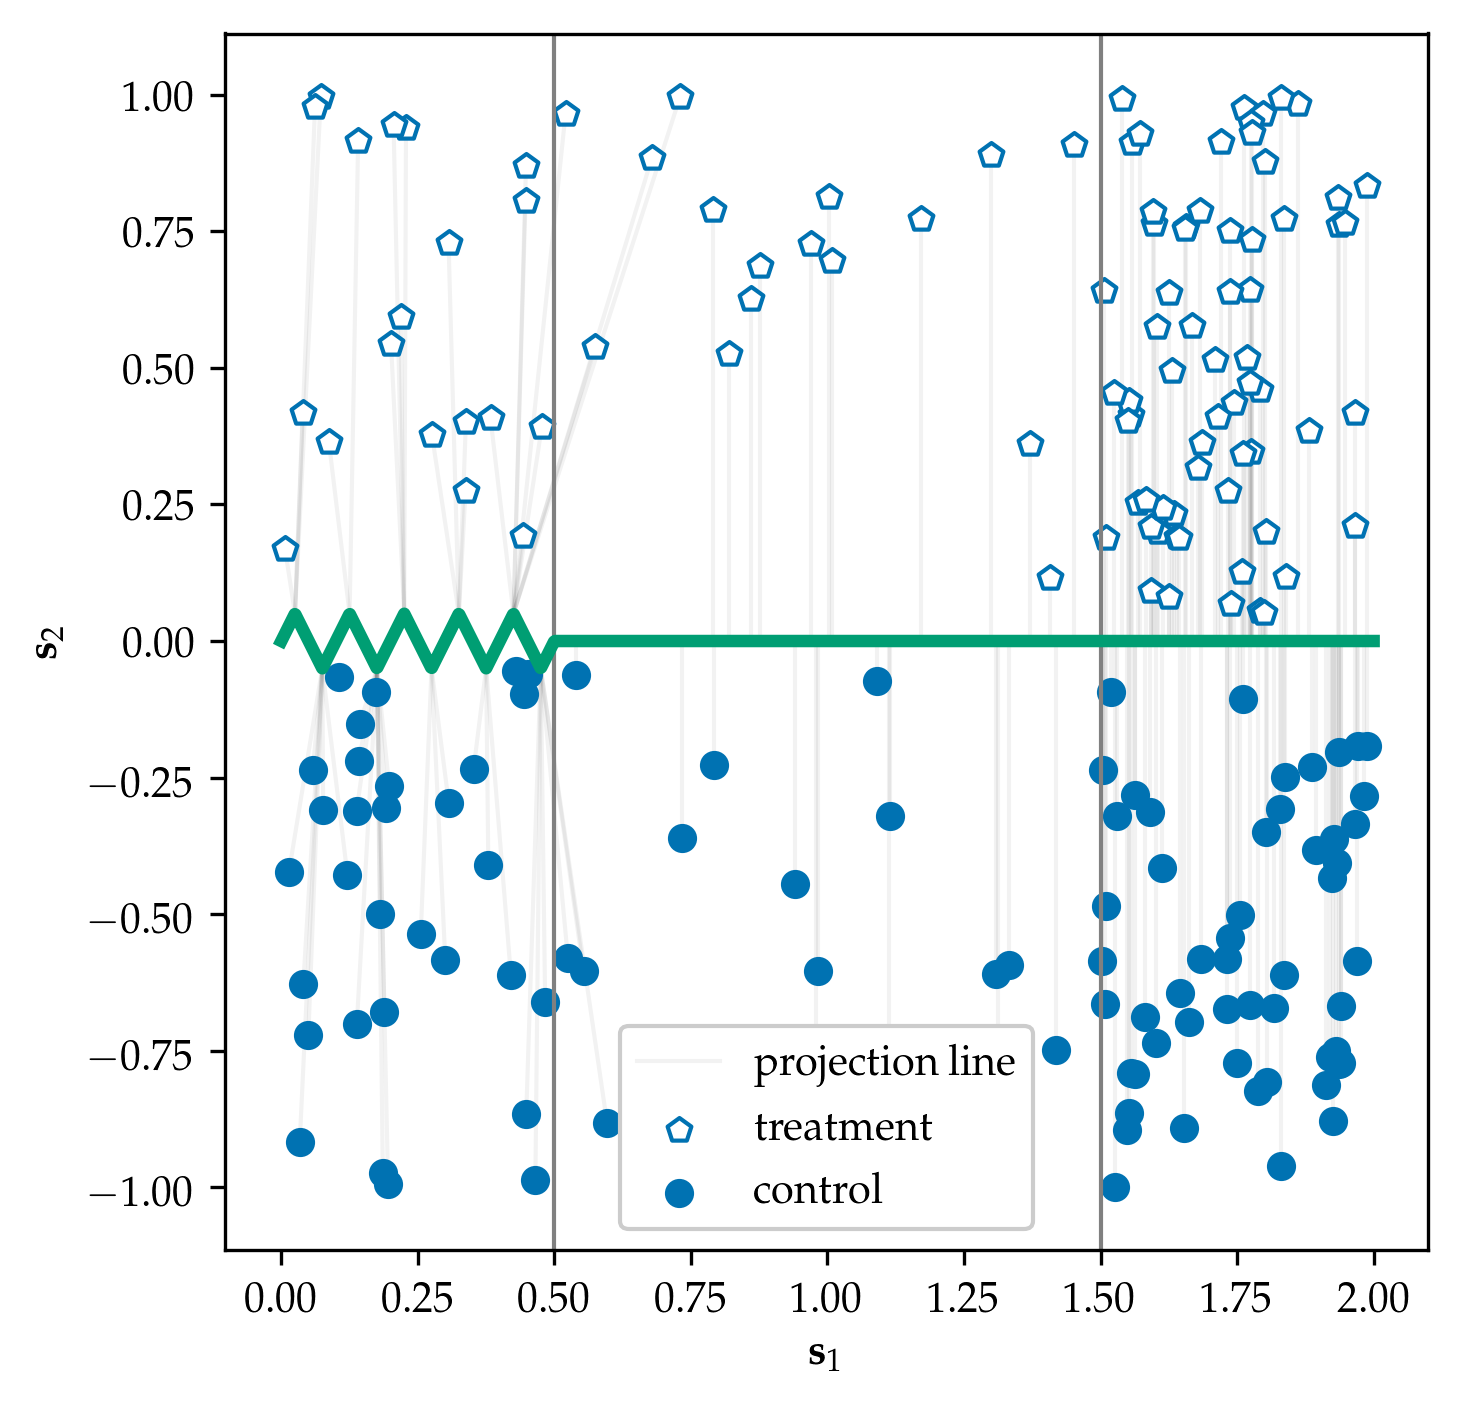
\includegraphics[height=0.35\textheight]{../figures/wiggly_boundaries_setup.png}
\caption{\label{fig:wiggly_boundaries_setup}Spatial positions of units and border for the wiggly border simulation of Section~\ref{sec:wiggly_border}. Projection lines for the projected finite population ATE are shown in light gray.}
\end{figure}
    

        We illustrate the above ATE estimators with a simulation.
200 units are placed in a square area delimited by spatial coordinates \(S_1 \in \cbr{0,2}\) and \(S_2 \in \cbr{-1, 1}\).
A border at \(S_2=0\) divides units vertically into a control and treatment region,
which are then further divided horizontally at \(S_1=0.5\) and \(S_1=1.5\) into three bands:

\begin{itemize}
\item
  The leftmost band \(S_1 < 0.5\) has a weak treatment effect.
\item
  The middle band \(0.5 \ge S_1 < 1.5\) has a much lower population density, and a stronger treatment effect.
\item
  The rightmost band \(S_1 \ge 1.5\), has a much higher population density, and a very strong treatment effect.
\end{itemize}

Furthermore, the border in the leftmost band is a triangular wave, to create ``wiggliness.''
We increase the number of wiggles from 0 to 1000 to observe the effect on the estimates.
The simulation setting is summarized in Table~\ref{table:wiggly_setup}.
We draw a single set of spatial coordinates, shown in Figure~\ref{fig:wiggly_boundaries_setup}, then draw 10,000 simulations of the outcomes \(Y\) from a Gaussian process with squared exponential kernel (\(\ell=0.4\), \(\sigma=0.5\)).
To units above the border we add a treatment effect \(\tau(S_1, S_2) = S_1\).



\begin{table}[tbp]
\centering
\begin{tabular}{llll}
\hline
& Left \(S_1< 0.5\) & Middle \(0.5 \ge S_1 < 1.5\) & Right \(1.5 \ge S_1\)\tabularnewline
\hline
\textbf{Border} & wiggly & straight & straight\tabularnewline
\textbf{Density} & low \(\rho=1.0\) & very low \(\rho=0.3\) & high \(\rho=2.0\)\tabularnewline
\(\taubold\) & weak & medium & strong\tabularnewline
\hline
\end{tabular}
\caption{Summary of wiggly border simulation setup. \label{table:wiggly_setup}}
\end{table}

        We fit the Gaussian process model \eqref{eq:spec2gp},
using the known hyperparameters of the covariance kernel and a weak prior on the mean parameter of each region,
and estimate the average treatment effect using the six methods proposed above.
In Figure \ref{fig:wiggly_boundaries_posteriors}(a) we show, for each estimator, the corresponding estimand and average posterior mean estimate evolving as the number of border wiggles increases.
The behavior of the posterior standard deviation is shown in Figure~\ref{fig:wiggly_boundaries_posteriors}(b).

\begin{figure}[tbp]
\centering
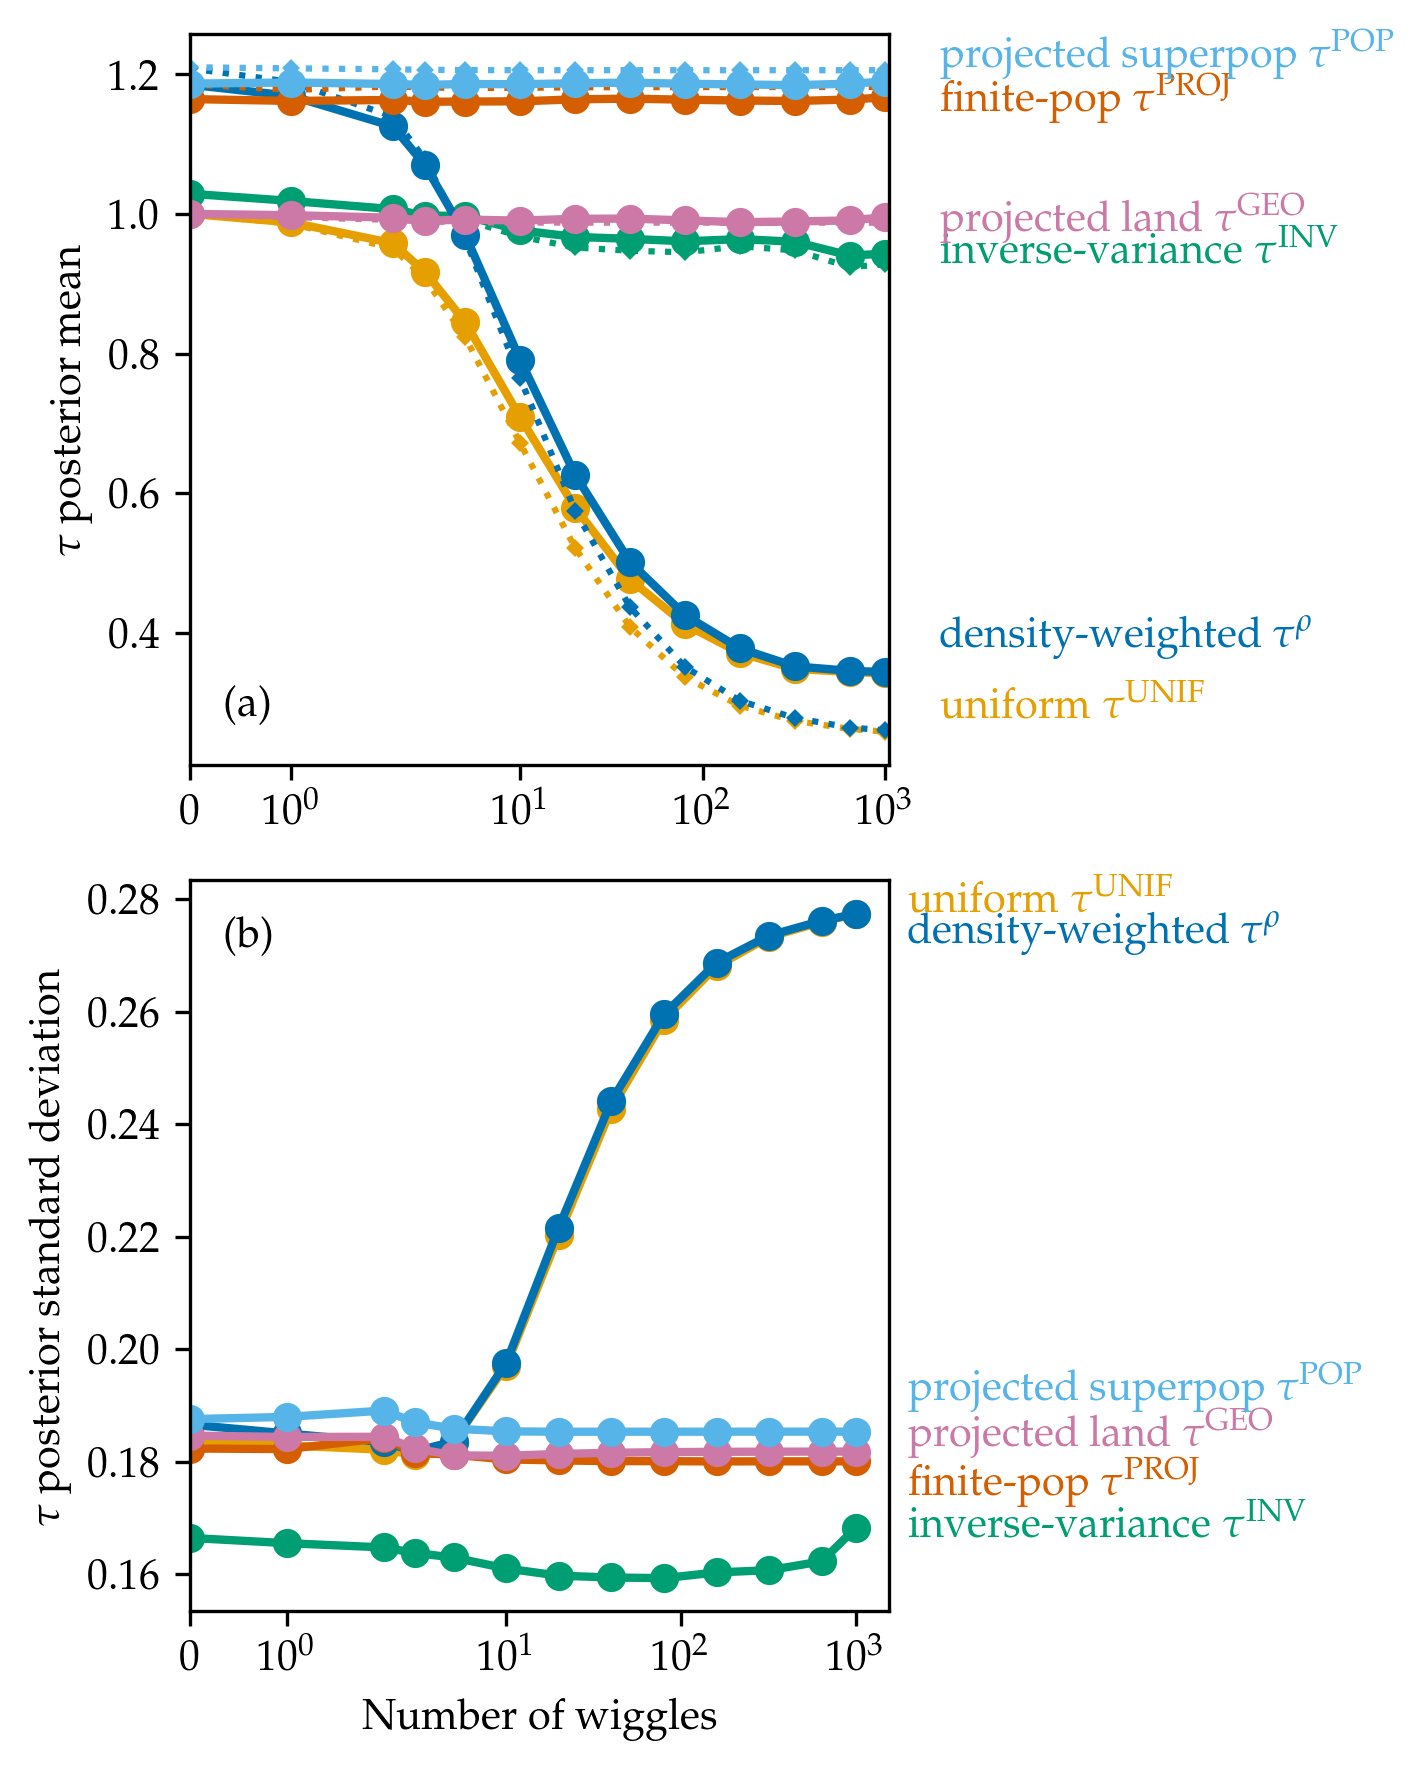
\includegraphics[height=0.4\textheight]{../figures/wiggly_boundaries_posteriors.png}
\caption{\label{fig:wiggly_boundaries_posteriors} Results of the simulations of Section~\ref{sec:wiggly_border}, showing for each ATE estimator as the leftmost section of the border gets wigglier (a) the estimate (posterior mean) averaged over 10,000 simulations with the corresponding estimand shown as a dotted line of the same color, and (b) the posterior standard deviation.}
\end{figure}
    
As the border is a straight line and \(\treatarea\) and \(\ctrolarea\) are rectangles,
and as the treatment effect does not depend on the vertical axis \(S_2\),
the density-weighted estimand \(\taurho\) equals the projected superpopulation estimand \(\taupop\),
and they are in fact both equal to the infinite-population average treatment effect.
Correspondingly, the posteriors of \(\taurho\) and \(\taupop\) are identical.
With 200 units, \(\taupop\) and the finite-population projected ATE \(\tauproj\) are also similar, but the latter has the advantage of not require estimating the population density.

The geometry- and geography-based ATE \(\unifavg\) and \(\taugeo\) are also equivalent when the border is a straight line.
They give equal weight to the sparsely populated middle band, which produces a lower estimate with higher variance than the posteriors of \(\taurho\) and \(\taupop\).

Lastly, the information-based inverse-variance estimand \(\invvar\) does not coincide with any others.
The estimand and mean estimate change slightly from 0 to 1 wiggles, but remains stable thereafter, demonstrating the robustness of this estimator to border topology.
Weighting by the inverse variance gives the lowest posterior variance within the class of ATEs under consideration, which can indeed be seen in Figure \ref{fig:wiggly_boundaries_posteriors}(b).

As we introduce wiggles into the leftmost band,
\(\taurho\) and \(\unifavg\) show their susceptibility to the border topology.
Proportionally more sentinels are packed into the leftmost section of the border,
upweighting the lower treatment effect of that band,
and resulting in a drop of the two estimates and estimands.
Meanwhile, \(\invvar\) remains stable despite the wiggles,
because the additional sentinels in the leftmost
band get automatically downweighted as their correlation rises.
The estimators that rely on projection
\(\tauproj\), \(\taugeo\), and \(\taupop\) also remain stable,
because the projected sentinels hardly move.
These robust estimands show only a slight displacement when the first wiggles are introduced,
caused by the presence of some sentinels nearer to the observed units.
    
\begin{figure}[ptb]
\centering
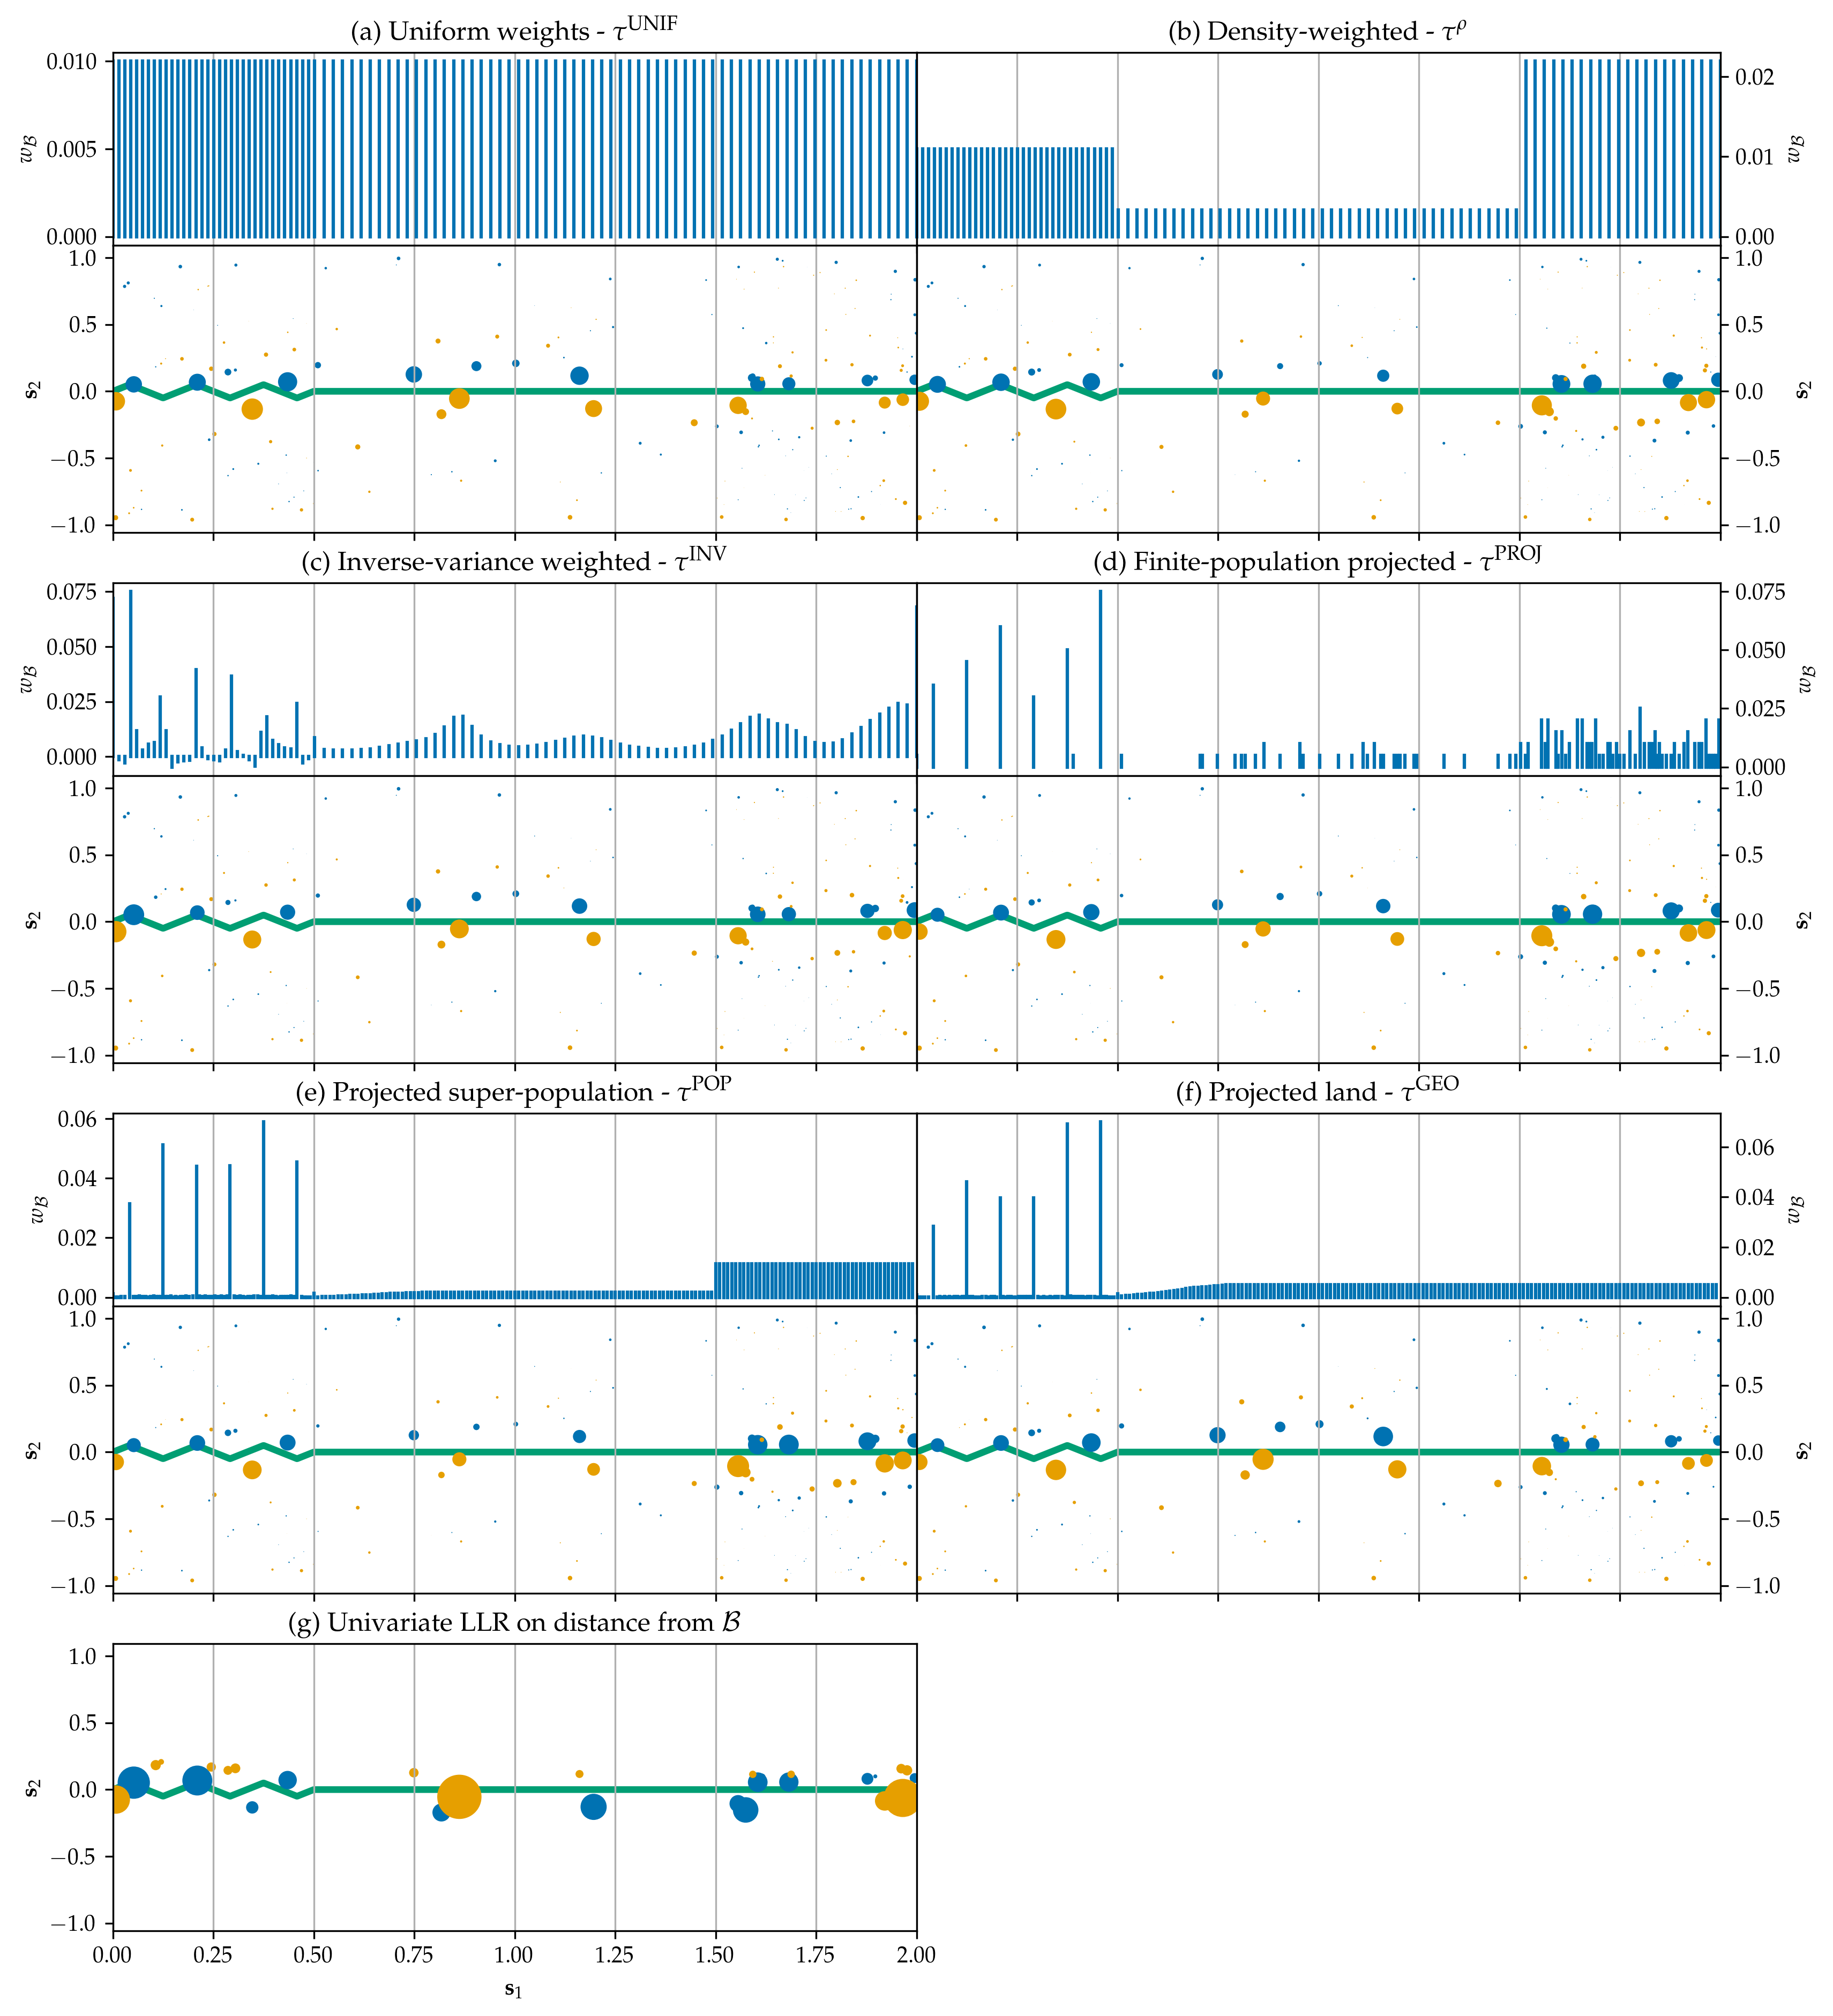
\includegraphics[width=\textwidth]{../figures/weight_functions.png}
\caption{\label{fig:weight_functions}Weight functions and induced weights on the observations for the six weight functions proposed in this paper. The weight function plots show the weight \(\weightb(\sentinel)\) against each sentinel's \(S_1\) coordinate. Sentinels with coinciding or nearly coinciding (within 0.005 of each other) coordinate \(S_1\) were merged and their weights summed. The induced weight plots show a circle for each unit, with the area of the circle proportional to its weight (\(\wt\) and \(\wc\) for treatment and control units respectively), and colored in blue for positive weights and orange for negative weights.}
\end{figure}
    

        In Figure~\ref{fig:weight_functions}(a-f), we illustrate the behavior of border weights \(\weightb(\sentinel)\) and unit weights (\(\wt\) and \(\wc\)) in this simulation setting with 3 wiggles.
Note how evenly spaced sentinels (for \(\unifavg\), \(\taurho\), and \(\invvar\)) are more densely packed along \(S_1\) in the leftmost area because of the zig-zagging border.
The inverse-variance weighted estimator border weights can be seen to respond to this change in the border topology, though it is difficult to interpret their oscillating behavior.
While these border-weights look unreasonable and unstable, the induced unit weights for \(\invvar\) are well-behaved, and in fact quite similar to those of the projected finite- and infinite-population estimators.
Furthermore, note that all estimators can give some small negative weights \(\wt\) to treatment units, and small positive weights \(\wc\) to control units.
For Gaussian processes, this can be understood in terms of the negative side-lobes of the equivalent kernel (see \cite{rasmussen2006gaussian} Section 2.6).
The high variance of \(\unifavg\) and \(\taugeo\) manifests itself as large weights given to a small number of units.
All other estimators spread the weights more evenly amongst the units near the border, which reduces their variance.
    


        For comparison, the weights placed on units by the projected 1D RDD are shown in Figure~\ref{fig:weight_functions}(g).
A triangular kernel in \(S_2\) was used with bandwidth selected using the MSE-minimizing method proposed by \cite{imbens2012optimal}.
The Projected 1D~RDD estimator can also be written as a linear combination of the observed outcomes \eqref{eq:unit_weights}, and the unit weight vectors can be derived as:
\begin{equation}
\begin{split}
\wt &= \hphantom{-} \Xmat_b (\Xmat_\treat\trans \Wmat_\treat \Xmat_\treat)^{-1} \Xmat_\treat\trans \Wmat_\treat \,, 
\text{ and}
\\
\wc &= - \Xmat_b (\Xmat_\ctrol\trans \Wmat_\ctrol \Xmat_\ctrol)^{-1} \Xmat_\ctrol\trans \Wmat_\ctrol \,, 
\end{split}
\eqlabel{eq:unit_weights_llr}
\end{equation}
where \(\Xmat_b = \del{1~0}\), \(\Xmat_\treat\) is the \(n_\treat \times 2\) design matrix with the first column filled with ones and the second column containing the distance from the border of each treatment unit, and \(\Wmat_\treat\) is an \(n_\treat \times n_\treat\) diagonal matrix where the \(i^\mathrm{th}\) diagonal element is the triangular kernel evaluated on the \(i^\mathrm{th}\) unit's distance from the border.
The \(\Xmat_\ctrol\) and \(\Wmat_\ctrol\) matrices are analogously defined for control units.
By construction, the unit weights drop to zero outside of the support of the kernel.
Within the support, Projected 1D RDD can also give negative weights to treatment units, and positive weights to control units.
This results from the negative influence on the prediction \(\widehat{y^*}\) at \(x^*\) that univariate linear regression can give to an observation \(Y_i\) at \(X_i\) sufficiently far away on the opposite side of the mean \(\overline{X}\) of all observations.
Strikingly, almost all of the positive weights are given to units in the rightmost treatment area that are closest to the border, and almost all the negative weights are given to units in the leftmost control area.
Consequently, any trend in the outcomes across \(S_1\) would confound the estimated treatment effect.

\end{document}
